\renewcommand{\theequation}{\theenumi}
\begin{enumerate}[label=\arabic*.,ref=\thesubsection.\theenumi]
\numberwithin{equation}{enumi}

\item $ABCD$ is a rectangle formed by the points $\vec{A} = \myvec{-1\\-1}, \vec{B} = \myvec{-1\\4}, \vec{C} = \myvec{5\\4}, \vec{D} = \myvec{5\\-1}$. $ \vec{P}, \vec{Q}, \vec{R}, \vec{S}$ are the mid points of $AB, BC, CD, DA$ respectively.  Is the quadrilateral $PQRS$ a 
\begin{enumerate}
\item square?
\item rectangle?
\item rhombus?
\end{enumerate}
\solution
Let the balanced version of (\ref{eq:solutions/chem/6ato balance}) be
\begin{align}
    \label{eq:solutions/chem/6abalanced}x_{1}HNO_{3}+ x_{2}Ca(OH)_{2}\to x_{3}Ca(NO_{3})_{2}+ x_{4}H_{2}O
\end{align}

which results in the following equations:
\begin{align}
    (x_{1}+ 2x_{2}-2x_{4}) H= 0\\
    (x_{1}-2x_{3}) N= 0\\
    (3x_{1}+ 2x_{2}-6x_{3}- x_{4}) O=0\\
    (x_{2}-x_{3}) Ca= 0
\end{align}

which can be expressed as
\begin{align}
    x_{1}+ 2x_{2}+ 0.x_{3} -2x_{4} = 0\\
    x_{1}+ 0.x_{2} -2x_{3} +0.x_{4}= 0\\
    3x_{1}+ 2x_{2}-6x_{3}- x_{4} =0\\
    0.x_{1} +x_{2}-x_{3} +0.x_{4}= 0
\end{align}

resulting in the matrix equation
\begin{align}
    \label{eq:solutions/chem/6a matrix}
    \myvec{1 & 2 & 0 & -2\\
           1 & 0 & -2 & 0\\
           3 & 2 & -6 & -1\\
           0 & 1 & -1 & 0}\vec{x}
           =\vec{0}
\end{align}

where,
\begin{align}
   \vec{x}= \myvec{x_{1}\\x_{2}\\x_{3}\\x_{4}}
\end{align}

(\ref{eq:solutions/chem/6a matrix}) can be reduced as follows:
\begin{align}
    \myvec{1 & 2 & 0 & -2\\
           1 & 0 & -2 & 0\\
           3 & 2 & -6 & -1\\
           0 & 1 & -1 & 0}
    \xleftrightarrow[R_{3}\leftarrow \frac{R_3}{3}-R_{1}]{R_{2}\leftarrow R_2- R_1}
    \myvec{1 & 2 & 0 & -2\\
           0 & -2 & -2 & 2\\
           0 & -\frac{4}{3} & -2 & \frac{5}{3}\\
           0 & 1 & -1 & 0}\\
    \xleftrightarrow{R_2 \leftarrow -\frac{R_2}{2}}
    \myvec{1 & 2 & 0 & -2\\
          0 & 1 & 1 & -1\\
          0 & -\frac{4}{3} & -2 & \frac{5}{3}\\
          0 & 1 & -1 & 0}\\
    \xleftrightarrow[R_4 \leftarrow R_4- R_2]{R_3 \leftarrow R_3 + \frac{4}{3}R_2}
    \myvec{1 & 2 & 0 & -2\\
           0 & 1 & 1 & -1\\
           0 & 0 & -\frac{2}{3} & \frac{1}{3}\\
           0 & 0 & -2 & 1}\\
    \xleftrightarrow[R_3 \leftarrow -\frac{3}{2}R_3]{R_1 \leftarrow R_1- 2R_2}
    \myvec{1 & 0 & -2 & 0\\
           0 & 1 & 1 & -1\\
           0 & 0 & 1 & -\frac{1}{2}\\
           0 & 0 & -2 & 1}\\
    \xleftrightarrow{R_4\leftarrow R_4 + 2R_3}
    \myvec{1 & 0 & -2 & 0\\
           0 & 1 & 1 & -1\\
           0 & 0 & 1 & -\frac{1}{2}\\
           0 & 0 & 0 & 0}\\
    \xleftrightarrow[R_2\leftarrow R_2-R_3]{R_1\leftarrow R_1 + 2R_3}
    \myvec{1 & 0 & 0 & -1\\
           0 & 1 & 0 & -\frac{1}{2}\\
           0 & 0 & 1 & -\frac{1}{2}\\
           0 & 0 & 0 & 0}
\end{align}

Thus,
\begin{align}
    x_1=x_4, x_2= \frac{1}{2}x_4, x_3=\frac{1}{2}x_4\\
    \implies \quad\vec{x}= x_4\myvec{1\\ \frac{1}{2}\\ \frac{1}{2}\\1} =\myvec{2\\1\\1\\2}
\end{align} 
by substituting $x_4= 2$.

\hfill\break
%\vspace{5mm} 
Hence, (\ref{eq:solutions/chem/6abalanced}) finally becomes
\begin{align}
    2HNO_{3}+ Ca(OH)_{2}\to Ca(NO_{3})_{2}+ 2H_{2}O
\end{align}

\item $ABCD$ is a cyclic quadrilateral with 
\begin{align}
\angle A &= 4y+20
\\
\angle B &= 3y-5
\\
\angle C &= -4x
\\
\angle D &= -7x+5
\end{align}
%
Find its angles.
\\
\solution
Let the balanced version of (\ref{eq:solutions/chem/6ato balance}) be
\begin{align}
    \label{eq:solutions/chem/6abalanced}x_{1}HNO_{3}+ x_{2}Ca(OH)_{2}\to x_{3}Ca(NO_{3})_{2}+ x_{4}H_{2}O
\end{align}

which results in the following equations:
\begin{align}
    (x_{1}+ 2x_{2}-2x_{4}) H= 0\\
    (x_{1}-2x_{3}) N= 0\\
    (3x_{1}+ 2x_{2}-6x_{3}- x_{4}) O=0\\
    (x_{2}-x_{3}) Ca= 0
\end{align}

which can be expressed as
\begin{align}
    x_{1}+ 2x_{2}+ 0.x_{3} -2x_{4} = 0\\
    x_{1}+ 0.x_{2} -2x_{3} +0.x_{4}= 0\\
    3x_{1}+ 2x_{2}-6x_{3}- x_{4} =0\\
    0.x_{1} +x_{2}-x_{3} +0.x_{4}= 0
\end{align}

resulting in the matrix equation
\begin{align}
    \label{eq:solutions/chem/6a matrix}
    \myvec{1 & 2 & 0 & -2\\
           1 & 0 & -2 & 0\\
           3 & 2 & -6 & -1\\
           0 & 1 & -1 & 0}\vec{x}
           =\vec{0}
\end{align}

where,
\begin{align}
   \vec{x}= \myvec{x_{1}\\x_{2}\\x_{3}\\x_{4}}
\end{align}

(\ref{eq:solutions/chem/6a matrix}) can be reduced as follows:
\begin{align}
    \myvec{1 & 2 & 0 & -2\\
           1 & 0 & -2 & 0\\
           3 & 2 & -6 & -1\\
           0 & 1 & -1 & 0}
    \xleftrightarrow[R_{3}\leftarrow \frac{R_3}{3}-R_{1}]{R_{2}\leftarrow R_2- R_1}
    \myvec{1 & 2 & 0 & -2\\
           0 & -2 & -2 & 2\\
           0 & -\frac{4}{3} & -2 & \frac{5}{3}\\
           0 & 1 & -1 & 0}\\
    \xleftrightarrow{R_2 \leftarrow -\frac{R_2}{2}}
    \myvec{1 & 2 & 0 & -2\\
          0 & 1 & 1 & -1\\
          0 & -\frac{4}{3} & -2 & \frac{5}{3}\\
          0 & 1 & -1 & 0}\\
    \xleftrightarrow[R_4 \leftarrow R_4- R_2]{R_3 \leftarrow R_3 + \frac{4}{3}R_2}
    \myvec{1 & 2 & 0 & -2\\
           0 & 1 & 1 & -1\\
           0 & 0 & -\frac{2}{3} & \frac{1}{3}\\
           0 & 0 & -2 & 1}\\
    \xleftrightarrow[R_3 \leftarrow -\frac{3}{2}R_3]{R_1 \leftarrow R_1- 2R_2}
    \myvec{1 & 0 & -2 & 0\\
           0 & 1 & 1 & -1\\
           0 & 0 & 1 & -\frac{1}{2}\\
           0 & 0 & -2 & 1}\\
    \xleftrightarrow{R_4\leftarrow R_4 + 2R_3}
    \myvec{1 & 0 & -2 & 0\\
           0 & 1 & 1 & -1\\
           0 & 0 & 1 & -\frac{1}{2}\\
           0 & 0 & 0 & 0}\\
    \xleftrightarrow[R_2\leftarrow R_2-R_3]{R_1\leftarrow R_1 + 2R_3}
    \myvec{1 & 0 & 0 & -1\\
           0 & 1 & 0 & -\frac{1}{2}\\
           0 & 0 & 1 & -\frac{1}{2}\\
           0 & 0 & 0 & 0}
\end{align}

Thus,
\begin{align}
    x_1=x_4, x_2= \frac{1}{2}x_4, x_3=\frac{1}{2}x_4\\
    \implies \quad\vec{x}= x_4\myvec{1\\ \frac{1}{2}\\ \frac{1}{2}\\1} =\myvec{2\\1\\1\\2}
\end{align} 
by substituting $x_4= 2$.

\hfill\break
%\vspace{5mm} 
Hence, (\ref{eq:solutions/chem/6abalanced}) finally becomes
\begin{align}
    2HNO_{3}+ Ca(OH)_{2}\to Ca(NO_{3})_{2}+ 2H_{2}O
\end{align}

\item Draw a quadrilateral in the Cartesian plane, whose vertices are \myvec{– 4\\ 5}, \myvec{0\\ 7}, \myvec{5\\ – 5} and \myvec{– 4\\ –2}. Also, find its area.
\\
\solution
Let the balanced version of (\ref{eq:solutions/chem/6ato balance}) be
\begin{align}
    \label{eq:solutions/chem/6abalanced}x_{1}HNO_{3}+ x_{2}Ca(OH)_{2}\to x_{3}Ca(NO_{3})_{2}+ x_{4}H_{2}O
\end{align}

which results in the following equations:
\begin{align}
    (x_{1}+ 2x_{2}-2x_{4}) H= 0\\
    (x_{1}-2x_{3}) N= 0\\
    (3x_{1}+ 2x_{2}-6x_{3}- x_{4}) O=0\\
    (x_{2}-x_{3}) Ca= 0
\end{align}

which can be expressed as
\begin{align}
    x_{1}+ 2x_{2}+ 0.x_{3} -2x_{4} = 0\\
    x_{1}+ 0.x_{2} -2x_{3} +0.x_{4}= 0\\
    3x_{1}+ 2x_{2}-6x_{3}- x_{4} =0\\
    0.x_{1} +x_{2}-x_{3} +0.x_{4}= 0
\end{align}

resulting in the matrix equation
\begin{align}
    \label{eq:solutions/chem/6a matrix}
    \myvec{1 & 2 & 0 & -2\\
           1 & 0 & -2 & 0\\
           3 & 2 & -6 & -1\\
           0 & 1 & -1 & 0}\vec{x}
           =\vec{0}
\end{align}

where,
\begin{align}
   \vec{x}= \myvec{x_{1}\\x_{2}\\x_{3}\\x_{4}}
\end{align}

(\ref{eq:solutions/chem/6a matrix}) can be reduced as follows:
\begin{align}
    \myvec{1 & 2 & 0 & -2\\
           1 & 0 & -2 & 0\\
           3 & 2 & -6 & -1\\
           0 & 1 & -1 & 0}
    \xleftrightarrow[R_{3}\leftarrow \frac{R_3}{3}-R_{1}]{R_{2}\leftarrow R_2- R_1}
    \myvec{1 & 2 & 0 & -2\\
           0 & -2 & -2 & 2\\
           0 & -\frac{4}{3} & -2 & \frac{5}{3}\\
           0 & 1 & -1 & 0}\\
    \xleftrightarrow{R_2 \leftarrow -\frac{R_2}{2}}
    \myvec{1 & 2 & 0 & -2\\
          0 & 1 & 1 & -1\\
          0 & -\frac{4}{3} & -2 & \frac{5}{3}\\
          0 & 1 & -1 & 0}\\
    \xleftrightarrow[R_4 \leftarrow R_4- R_2]{R_3 \leftarrow R_3 + \frac{4}{3}R_2}
    \myvec{1 & 2 & 0 & -2\\
           0 & 1 & 1 & -1\\
           0 & 0 & -\frac{2}{3} & \frac{1}{3}\\
           0 & 0 & -2 & 1}\\
    \xleftrightarrow[R_3 \leftarrow -\frac{3}{2}R_3]{R_1 \leftarrow R_1- 2R_2}
    \myvec{1 & 0 & -2 & 0\\
           0 & 1 & 1 & -1\\
           0 & 0 & 1 & -\frac{1}{2}\\
           0 & 0 & -2 & 1}\\
    \xleftrightarrow{R_4\leftarrow R_4 + 2R_3}
    \myvec{1 & 0 & -2 & 0\\
           0 & 1 & 1 & -1\\
           0 & 0 & 1 & -\frac{1}{2}\\
           0 & 0 & 0 & 0}\\
    \xleftrightarrow[R_2\leftarrow R_2-R_3]{R_1\leftarrow R_1 + 2R_3}
    \myvec{1 & 0 & 0 & -1\\
           0 & 1 & 0 & -\frac{1}{2}\\
           0 & 0 & 1 & -\frac{1}{2}\\
           0 & 0 & 0 & 0}
\end{align}

Thus,
\begin{align}
    x_1=x_4, x_2= \frac{1}{2}x_4, x_3=\frac{1}{2}x_4\\
    \implies \quad\vec{x}= x_4\myvec{1\\ \frac{1}{2}\\ \frac{1}{2}\\1} =\myvec{2\\1\\1\\2}
\end{align} 
by substituting $x_4= 2$.

\hfill\break
%\vspace{5mm} 
Hence, (\ref{eq:solutions/chem/6abalanced}) finally becomes
\begin{align}
    2HNO_{3}+ Ca(OH)_{2}\to Ca(NO_{3})_{2}+ 2H_{2}O
\end{align}


\item Find the area of a rhombus if its vertices are 
\begin{align}
\vec{P} &= \myvec{3\\0}, \vec{Q} =\myvec{4\\5},
\\
\vec{R} &= \myvec{-1\\4}, \vec{S} = \myvec{-2\\-1} 
\end{align}
taken in order.
\\
\solution
Let the balanced version of (\ref{eq:solutions/chem/6ato balance}) be
\begin{align}
    \label{eq:solutions/chem/6abalanced}x_{1}HNO_{3}+ x_{2}Ca(OH)_{2}\to x_{3}Ca(NO_{3})_{2}+ x_{4}H_{2}O
\end{align}

which results in the following equations:
\begin{align}
    (x_{1}+ 2x_{2}-2x_{4}) H= 0\\
    (x_{1}-2x_{3}) N= 0\\
    (3x_{1}+ 2x_{2}-6x_{3}- x_{4}) O=0\\
    (x_{2}-x_{3}) Ca= 0
\end{align}

which can be expressed as
\begin{align}
    x_{1}+ 2x_{2}+ 0.x_{3} -2x_{4} = 0\\
    x_{1}+ 0.x_{2} -2x_{3} +0.x_{4}= 0\\
    3x_{1}+ 2x_{2}-6x_{3}- x_{4} =0\\
    0.x_{1} +x_{2}-x_{3} +0.x_{4}= 0
\end{align}

resulting in the matrix equation
\begin{align}
    \label{eq:solutions/chem/6a matrix}
    \myvec{1 & 2 & 0 & -2\\
           1 & 0 & -2 & 0\\
           3 & 2 & -6 & -1\\
           0 & 1 & -1 & 0}\vec{x}
           =\vec{0}
\end{align}

where,
\begin{align}
   \vec{x}= \myvec{x_{1}\\x_{2}\\x_{3}\\x_{4}}
\end{align}

(\ref{eq:solutions/chem/6a matrix}) can be reduced as follows:
\begin{align}
    \myvec{1 & 2 & 0 & -2\\
           1 & 0 & -2 & 0\\
           3 & 2 & -6 & -1\\
           0 & 1 & -1 & 0}
    \xleftrightarrow[R_{3}\leftarrow \frac{R_3}{3}-R_{1}]{R_{2}\leftarrow R_2- R_1}
    \myvec{1 & 2 & 0 & -2\\
           0 & -2 & -2 & 2\\
           0 & -\frac{4}{3} & -2 & \frac{5}{3}\\
           0 & 1 & -1 & 0}\\
    \xleftrightarrow{R_2 \leftarrow -\frac{R_2}{2}}
    \myvec{1 & 2 & 0 & -2\\
          0 & 1 & 1 & -1\\
          0 & -\frac{4}{3} & -2 & \frac{5}{3}\\
          0 & 1 & -1 & 0}\\
    \xleftrightarrow[R_4 \leftarrow R_4- R_2]{R_3 \leftarrow R_3 + \frac{4}{3}R_2}
    \myvec{1 & 2 & 0 & -2\\
           0 & 1 & 1 & -1\\
           0 & 0 & -\frac{2}{3} & \frac{1}{3}\\
           0 & 0 & -2 & 1}\\
    \xleftrightarrow[R_3 \leftarrow -\frac{3}{2}R_3]{R_1 \leftarrow R_1- 2R_2}
    \myvec{1 & 0 & -2 & 0\\
           0 & 1 & 1 & -1\\
           0 & 0 & 1 & -\frac{1}{2}\\
           0 & 0 & -2 & 1}\\
    \xleftrightarrow{R_4\leftarrow R_4 + 2R_3}
    \myvec{1 & 0 & -2 & 0\\
           0 & 1 & 1 & -1\\
           0 & 0 & 1 & -\frac{1}{2}\\
           0 & 0 & 0 & 0}\\
    \xleftrightarrow[R_2\leftarrow R_2-R_3]{R_1\leftarrow R_1 + 2R_3}
    \myvec{1 & 0 & 0 & -1\\
           0 & 1 & 0 & -\frac{1}{2}\\
           0 & 0 & 1 & -\frac{1}{2}\\
           0 & 0 & 0 & 0}
\end{align}

Thus,
\begin{align}
    x_1=x_4, x_2= \frac{1}{2}x_4, x_3=\frac{1}{2}x_4\\
    \implies \quad\vec{x}= x_4\myvec{1\\ \frac{1}{2}\\ \frac{1}{2}\\1} =\myvec{2\\1\\1\\2}
\end{align} 
by substituting $x_4= 2$.

\hfill\break
%\vspace{5mm} 
Hence, (\ref{eq:solutions/chem/6abalanced}) finally becomes
\begin{align}
    2HNO_{3}+ Ca(OH)_{2}\to Ca(NO_{3})_{2}+ 2H_{2}O
\end{align}

\item Without using distance formula, show that points \myvec{– 2\\ – 1}, \myvec{4\\ 0}, \myvec{3\\ 3} and \myvec{–3\\ 2} are the vertices of a parallelogram.
\\
\solution
The following python code plots Fig.\ref{fig:2.2.5_qfour}.
	\begin{lstlisting}
	./solutions/5/codes/quadrilateral/q4.py
	\end{lstlisting}
	

	\begin{align}
\because	\vec{A - B}&=\vec{D - C}
	\\
	\vec{A - D}&=\vec{B - C},
	\end{align}
	
	$AB \parallel CD$ and $AD \parallel BC$.  Hence, $ABCD$ is a $\parallel$gm.
	\begin{figure}[!ht]
	\centering
	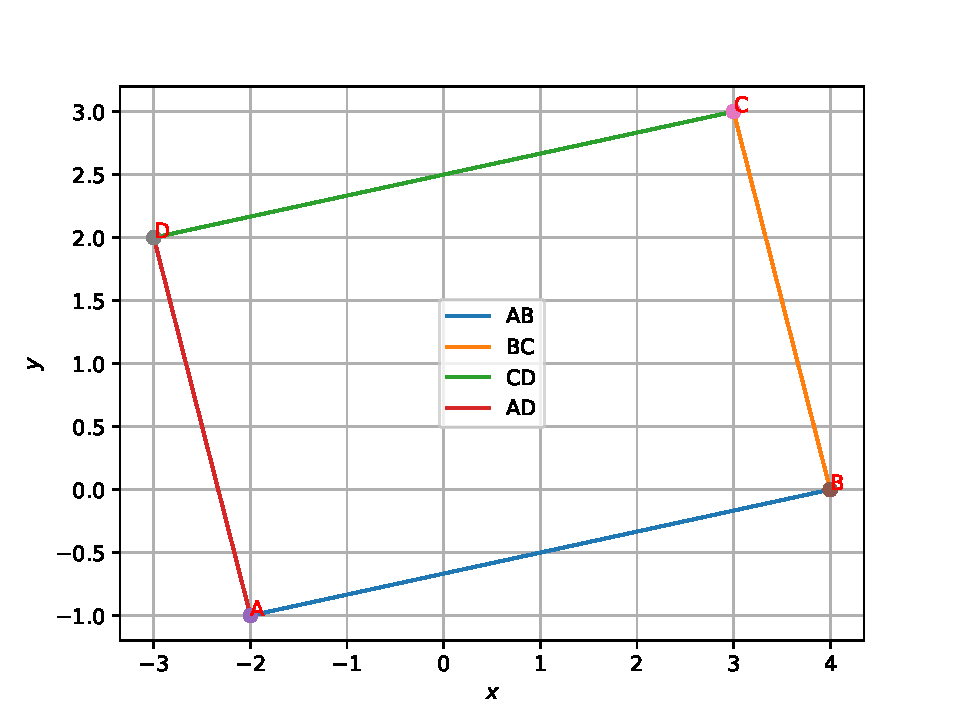
\includegraphics[width=\columnwidth]{./solutions/5/figs/quadrilateral/q4.eps}
	\caption{}
	\label{fig:2.2.5_qfour}	
	\end{figure}

\item  Find the area of the quadrilateral whose vertices, taken in order, are 
 \myvec{-4\\2},  \myvec{-3\\-5},  \myvec{3\\-2},  \myvec{2\\3}. 
\\
\solution
Let the balanced version of (\ref{eq:solutions/chem/6ato balance}) be
\begin{align}
    \label{eq:solutions/chem/6abalanced}x_{1}HNO_{3}+ x_{2}Ca(OH)_{2}\to x_{3}Ca(NO_{3})_{2}+ x_{4}H_{2}O
\end{align}

which results in the following equations:
\begin{align}
    (x_{1}+ 2x_{2}-2x_{4}) H= 0\\
    (x_{1}-2x_{3}) N= 0\\
    (3x_{1}+ 2x_{2}-6x_{3}- x_{4}) O=0\\
    (x_{2}-x_{3}) Ca= 0
\end{align}

which can be expressed as
\begin{align}
    x_{1}+ 2x_{2}+ 0.x_{3} -2x_{4} = 0\\
    x_{1}+ 0.x_{2} -2x_{3} +0.x_{4}= 0\\
    3x_{1}+ 2x_{2}-6x_{3}- x_{4} =0\\
    0.x_{1} +x_{2}-x_{3} +0.x_{4}= 0
\end{align}

resulting in the matrix equation
\begin{align}
    \label{eq:solutions/chem/6a matrix}
    \myvec{1 & 2 & 0 & -2\\
           1 & 0 & -2 & 0\\
           3 & 2 & -6 & -1\\
           0 & 1 & -1 & 0}\vec{x}
           =\vec{0}
\end{align}

where,
\begin{align}
   \vec{x}= \myvec{x_{1}\\x_{2}\\x_{3}\\x_{4}}
\end{align}

(\ref{eq:solutions/chem/6a matrix}) can be reduced as follows:
\begin{align}
    \myvec{1 & 2 & 0 & -2\\
           1 & 0 & -2 & 0\\
           3 & 2 & -6 & -1\\
           0 & 1 & -1 & 0}
    \xleftrightarrow[R_{3}\leftarrow \frac{R_3}{3}-R_{1}]{R_{2}\leftarrow R_2- R_1}
    \myvec{1 & 2 & 0 & -2\\
           0 & -2 & -2 & 2\\
           0 & -\frac{4}{3} & -2 & \frac{5}{3}\\
           0 & 1 & -1 & 0}\\
    \xleftrightarrow{R_2 \leftarrow -\frac{R_2}{2}}
    \myvec{1 & 2 & 0 & -2\\
          0 & 1 & 1 & -1\\
          0 & -\frac{4}{3} & -2 & \frac{5}{3}\\
          0 & 1 & -1 & 0}\\
    \xleftrightarrow[R_4 \leftarrow R_4- R_2]{R_3 \leftarrow R_3 + \frac{4}{3}R_2}
    \myvec{1 & 2 & 0 & -2\\
           0 & 1 & 1 & -1\\
           0 & 0 & -\frac{2}{3} & \frac{1}{3}\\
           0 & 0 & -2 & 1}\\
    \xleftrightarrow[R_3 \leftarrow -\frac{3}{2}R_3]{R_1 \leftarrow R_1- 2R_2}
    \myvec{1 & 0 & -2 & 0\\
           0 & 1 & 1 & -1\\
           0 & 0 & 1 & -\frac{1}{2}\\
           0 & 0 & -2 & 1}\\
    \xleftrightarrow{R_4\leftarrow R_4 + 2R_3}
    \myvec{1 & 0 & -2 & 0\\
           0 & 1 & 1 & -1\\
           0 & 0 & 1 & -\frac{1}{2}\\
           0 & 0 & 0 & 0}\\
    \xleftrightarrow[R_2\leftarrow R_2-R_3]{R_1\leftarrow R_1 + 2R_3}
    \myvec{1 & 0 & 0 & -1\\
           0 & 1 & 0 & -\frac{1}{2}\\
           0 & 0 & 1 & -\frac{1}{2}\\
           0 & 0 & 0 & 0}
\end{align}

Thus,
\begin{align}
    x_1=x_4, x_2= \frac{1}{2}x_4, x_3=\frac{1}{2}x_4\\
    \implies \quad\vec{x}= x_4\myvec{1\\ \frac{1}{2}\\ \frac{1}{2}\\1} =\myvec{2\\1\\1\\2}
\end{align} 
by substituting $x_4= 2$.

\hfill\break
%\vspace{5mm} 
Hence, (\ref{eq:solutions/chem/6abalanced}) finally becomes
\begin{align}
    2HNO_{3}+ Ca(OH)_{2}\to Ca(NO_{3})_{2}+ 2H_{2}O
\end{align}

\item The two opposite vertices of a square are \myvec{-1\\2},  \myvec{3\\2}. Find the coordinates of the other two vertices.
\\
\solution
\begin{align}
\myvec{1\\1} &= \sqrt{2}\myvec{\frac{1}{\sqrt{2}}\\ \frac{1}{\sqrt{2}}}
\\
&= \sqrt{2}\myvec{\cos 45\degree \\ \sin 45\degree}
\label{eq:3.4.7}
\end{align}
In the above, the modulus is $\norm{\myvec{1\\1}}=\sqrt{2}$ and the argument is $45 \degree$.
Similarly, 
\begin{align}
\myvec{1\\-1} &= \sqrt{2}\myvec{\cos 45\degree \\ -\sin 45\degree}
\\
\implies \myvec{1\\-1}^{-1} &= \frac{1}{\sqrt{2}}\myvec{\cos 45\degree \\ \sin 45\degree}
\end{align}
Using the matrix representation, 
\begin{align}
\frac{\myvec{1\\1}}{\myvec{1\\-1}} &= \myvec{\cos45\degree&-\sin45\degree\\\sin45\degree&\cos45\degree}
\nonumber \\
&\quad \times  \myvec{\cos45\degree&-\sin45\degree\\\sin45\degree&\cos45\degree}
\myvec{1\\0}
\\
 &= \myvec{\cos 90\degree\\ \sin 90\degree}= 1 \phase{90\degree}\end{align}
%
In general, if
\begin{align}
\vec{z}_1 &= r_1\myvec{\cos\theta_1\\\sin\theta_1}, \vec{z}_2 = r_2\myvec{\cos\theta_2\\\sin\theta_2},
\\
\vec{z}_1\vec{z}_2 &= r_1r_2\myvec{\cos(\theta_1+\theta_2)\\\sin(\theta_1+\theta_2)}.
\end{align}
Similarly, from \eqref{eq:3.4.7},
\begin{align}
\frac{1}{\myvec{1\\1}} &= \frac{1}{\sqrt{2}}\myvec{\cos 45\degree \\ -\sin 45\degree}
\\
&= \frac{1}{\sqrt{2}}\phase{-45\degree}
\end{align}

\item Find the area of a parallelogram whose adjacent sides are given by the vectors \myvec{3\\1\\4} and \myvec{1\\-1\\1}.
\\
\solution
Let the balanced version of (\ref{eq:solutions/chem/6ato balance}) be
\begin{align}
    \label{eq:solutions/chem/6abalanced}x_{1}HNO_{3}+ x_{2}Ca(OH)_{2}\to x_{3}Ca(NO_{3})_{2}+ x_{4}H_{2}O
\end{align}

which results in the following equations:
\begin{align}
    (x_{1}+ 2x_{2}-2x_{4}) H= 0\\
    (x_{1}-2x_{3}) N= 0\\
    (3x_{1}+ 2x_{2}-6x_{3}- x_{4}) O=0\\
    (x_{2}-x_{3}) Ca= 0
\end{align}

which can be expressed as
\begin{align}
    x_{1}+ 2x_{2}+ 0.x_{3} -2x_{4} = 0\\
    x_{1}+ 0.x_{2} -2x_{3} +0.x_{4}= 0\\
    3x_{1}+ 2x_{2}-6x_{3}- x_{4} =0\\
    0.x_{1} +x_{2}-x_{3} +0.x_{4}= 0
\end{align}

resulting in the matrix equation
\begin{align}
    \label{eq:solutions/chem/6a matrix}
    \myvec{1 & 2 & 0 & -2\\
           1 & 0 & -2 & 0\\
           3 & 2 & -6 & -1\\
           0 & 1 & -1 & 0}\vec{x}
           =\vec{0}
\end{align}

where,
\begin{align}
   \vec{x}= \myvec{x_{1}\\x_{2}\\x_{3}\\x_{4}}
\end{align}

(\ref{eq:solutions/chem/6a matrix}) can be reduced as follows:
\begin{align}
    \myvec{1 & 2 & 0 & -2\\
           1 & 0 & -2 & 0\\
           3 & 2 & -6 & -1\\
           0 & 1 & -1 & 0}
    \xleftrightarrow[R_{3}\leftarrow \frac{R_3}{3}-R_{1}]{R_{2}\leftarrow R_2- R_1}
    \myvec{1 & 2 & 0 & -2\\
           0 & -2 & -2 & 2\\
           0 & -\frac{4}{3} & -2 & \frac{5}{3}\\
           0 & 1 & -1 & 0}\\
    \xleftrightarrow{R_2 \leftarrow -\frac{R_2}{2}}
    \myvec{1 & 2 & 0 & -2\\
          0 & 1 & 1 & -1\\
          0 & -\frac{4}{3} & -2 & \frac{5}{3}\\
          0 & 1 & -1 & 0}\\
    \xleftrightarrow[R_4 \leftarrow R_4- R_2]{R_3 \leftarrow R_3 + \frac{4}{3}R_2}
    \myvec{1 & 2 & 0 & -2\\
           0 & 1 & 1 & -1\\
           0 & 0 & -\frac{2}{3} & \frac{1}{3}\\
           0 & 0 & -2 & 1}\\
    \xleftrightarrow[R_3 \leftarrow -\frac{3}{2}R_3]{R_1 \leftarrow R_1- 2R_2}
    \myvec{1 & 0 & -2 & 0\\
           0 & 1 & 1 & -1\\
           0 & 0 & 1 & -\frac{1}{2}\\
           0 & 0 & -2 & 1}\\
    \xleftrightarrow{R_4\leftarrow R_4 + 2R_3}
    \myvec{1 & 0 & -2 & 0\\
           0 & 1 & 1 & -1\\
           0 & 0 & 1 & -\frac{1}{2}\\
           0 & 0 & 0 & 0}\\
    \xleftrightarrow[R_2\leftarrow R_2-R_3]{R_1\leftarrow R_1 + 2R_3}
    \myvec{1 & 0 & 0 & -1\\
           0 & 1 & 0 & -\frac{1}{2}\\
           0 & 0 & 1 & -\frac{1}{2}\\
           0 & 0 & 0 & 0}
\end{align}

Thus,
\begin{align}
    x_1=x_4, x_2= \frac{1}{2}x_4, x_3=\frac{1}{2}x_4\\
    \implies \quad\vec{x}= x_4\myvec{1\\ \frac{1}{2}\\ \frac{1}{2}\\1} =\myvec{2\\1\\1\\2}
\end{align} 
by substituting $x_4= 2$.

\hfill\break
%\vspace{5mm} 
Hence, (\ref{eq:solutions/chem/6abalanced}) finally becomes
\begin{align}
    2HNO_{3}+ Ca(OH)_{2}\to Ca(NO_{3})_{2}+ 2H_{2}O
\end{align}

\item Find the area of a parallelogram whose adjacent sides are determined by the vectors $\vec{a} = \myvec{1\\-1\\3}$ and $\vec{b}=\myvec{2\\-7\\1}$.
\item Find the area of a rectangle $ABCD$ with vertices
$\vec{A} = \myvec{-1\\\frac{1}{2}\\ 4},
 \vec{B} = \myvec{1\\\frac{1}{2}\\ 4},
\vec{C} = \myvec{1\\-\frac{1}{2}\\ 4},
\vec{D} = \myvec{-1\\-\frac{1}{2}\\ 4}.
$
\\
\solution
Let the balanced version of (\ref{eq:solutions/chem/6ato balance}) be
\begin{align}
    \label{eq:solutions/chem/6abalanced}x_{1}HNO_{3}+ x_{2}Ca(OH)_{2}\to x_{3}Ca(NO_{3})_{2}+ x_{4}H_{2}O
\end{align}

which results in the following equations:
\begin{align}
    (x_{1}+ 2x_{2}-2x_{4}) H= 0\\
    (x_{1}-2x_{3}) N= 0\\
    (3x_{1}+ 2x_{2}-6x_{3}- x_{4}) O=0\\
    (x_{2}-x_{3}) Ca= 0
\end{align}

which can be expressed as
\begin{align}
    x_{1}+ 2x_{2}+ 0.x_{3} -2x_{4} = 0\\
    x_{1}+ 0.x_{2} -2x_{3} +0.x_{4}= 0\\
    3x_{1}+ 2x_{2}-6x_{3}- x_{4} =0\\
    0.x_{1} +x_{2}-x_{3} +0.x_{4}= 0
\end{align}

resulting in the matrix equation
\begin{align}
    \label{eq:solutions/chem/6a matrix}
    \myvec{1 & 2 & 0 & -2\\
           1 & 0 & -2 & 0\\
           3 & 2 & -6 & -1\\
           0 & 1 & -1 & 0}\vec{x}
           =\vec{0}
\end{align}

where,
\begin{align}
   \vec{x}= \myvec{x_{1}\\x_{2}\\x_{3}\\x_{4}}
\end{align}

(\ref{eq:solutions/chem/6a matrix}) can be reduced as follows:
\begin{align}
    \myvec{1 & 2 & 0 & -2\\
           1 & 0 & -2 & 0\\
           3 & 2 & -6 & -1\\
           0 & 1 & -1 & 0}
    \xleftrightarrow[R_{3}\leftarrow \frac{R_3}{3}-R_{1}]{R_{2}\leftarrow R_2- R_1}
    \myvec{1 & 2 & 0 & -2\\
           0 & -2 & -2 & 2\\
           0 & -\frac{4}{3} & -2 & \frac{5}{3}\\
           0 & 1 & -1 & 0}\\
    \xleftrightarrow{R_2 \leftarrow -\frac{R_2}{2}}
    \myvec{1 & 2 & 0 & -2\\
          0 & 1 & 1 & -1\\
          0 & -\frac{4}{3} & -2 & \frac{5}{3}\\
          0 & 1 & -1 & 0}\\
    \xleftrightarrow[R_4 \leftarrow R_4- R_2]{R_3 \leftarrow R_3 + \frac{4}{3}R_2}
    \myvec{1 & 2 & 0 & -2\\
           0 & 1 & 1 & -1\\
           0 & 0 & -\frac{2}{3} & \frac{1}{3}\\
           0 & 0 & -2 & 1}\\
    \xleftrightarrow[R_3 \leftarrow -\frac{3}{2}R_3]{R_1 \leftarrow R_1- 2R_2}
    \myvec{1 & 0 & -2 & 0\\
           0 & 1 & 1 & -1\\
           0 & 0 & 1 & -\frac{1}{2}\\
           0 & 0 & -2 & 1}\\
    \xleftrightarrow{R_4\leftarrow R_4 + 2R_3}
    \myvec{1 & 0 & -2 & 0\\
           0 & 1 & 1 & -1\\
           0 & 0 & 1 & -\frac{1}{2}\\
           0 & 0 & 0 & 0}\\
    \xleftrightarrow[R_2\leftarrow R_2-R_3]{R_1\leftarrow R_1 + 2R_3}
    \myvec{1 & 0 & 0 & -1\\
           0 & 1 & 0 & -\frac{1}{2}\\
           0 & 0 & 1 & -\frac{1}{2}\\
           0 & 0 & 0 & 0}
\end{align}

Thus,
\begin{align}
    x_1=x_4, x_2= \frac{1}{2}x_4, x_3=\frac{1}{2}x_4\\
    \implies \quad\vec{x}= x_4\myvec{1\\ \frac{1}{2}\\ \frac{1}{2}\\1} =\myvec{2\\1\\1\\2}
\end{align} 
by substituting $x_4= 2$.

\hfill\break
%\vspace{5mm} 
Hence, (\ref{eq:solutions/chem/6abalanced}) finally becomes
\begin{align}
    2HNO_{3}+ Ca(OH)_{2}\to Ca(NO_{3})_{2}+ 2H_{2}O
\end{align}

\item The two adjacent sides of a parallelogram are \myvec{2\\ -4 \\ -5} and  \myvec{1\\-2\\ -3}. Find the unit vector parallel to its diagonal.  Also, find its area.
%
%
\end{enumerate}
%
